\documentclass[12pt,twoside]{article}
\usepackage{amsfonts,amsmath,amssymb,amsthm,color,arydshln}
\usepackage{epsfig}
\usepackage{arydshln}
\usepackage{mathtools}
\textheight=19.9cm \textwidth=14.8cm \topmargin=0.5cm
\oddsidemargin=1cm \evensidemargin=1cm

\everymath{\displaystyle}
\def\l{\left}
\def\r{\right}
\def\theequation{\arabic{section}.\arabic{equation}}
\newcommand{\bb}[1]{\begin{equation}\label{#1}}
\newcommand{\ee}{\end{equation}}
\newcommand{\bbb}{\begin{eqnarray}}
\newcommand{\eee}{\end{eqnarray}}
\newcommand{\bbbb}{\begin{eqnarray*}}
\newcommand{\eeee}{\end{eqnarray*}}
\newcommand{\nnn}{\nonumber}
\newcommand{\no}{\noindent}
\newcommand{\tT}{\intercal}
\def\TT{\mathbb{T}}
\def\RR{\mathbb{R}}
\def\CC{\mathbb{C}}
\def\DD{{\cal D}}
\def\OO{{\cal{O}}}
\def\R#1{$(\ref{#1})$}
\def\dia{\mbox{diamond-$\alpha$}}
\def\diast{{\diamondsuit_{\alpha}}}
\definecolor{green1}{rgb}{0.1,0.5,0.0}
\definecolor{blue1}{RGB}{51,78,125}
\definecolor{brown}{RGB}{220,90,49}
\definecolor{red1}{rgb}{0.8,0.1,0.0}
\definecolor{orange}{rgb}{1,0.5,0}
\definecolor{gray2}{rgb}{0.8,0.8,0.8}
\newcommand{\darkgreen}{\color{green1}}
\newcommand{\darkblue}{\color{blue1}}
\newcommand{\darkred}{\color{red1}}
\newcommand{\orange}{\color{orange}}
\newcommand{\blue}{\color{blue}}
\newcommand{\gray}{\color{gray2}}
\newcommand{\red}{\color{red}}
\newtheorem{Theorem}{Theorem}[section]
\newtheorem{Lemma}[Theorem]{Lemma}
\newtheorem{Corollary}[Theorem]{Corollary}
\newtheorem{Proposition}[Theorem]{Propoision}
\newtheorem{Definition}[Theorem]{Definition}
\newtheorem{remark}[Theorem]{Remark}
\usepackage[utf8]{inputenc}
\usepackage[english]{babel}
\usepackage{graphicx}
\graphicspath{ {images/} }

 
\newtheorem{theorem}{Theorem}[section]
\newtheorem{corollary}{Corollary}[theorem]
\newtheorem{lemma}[theorem]{Lemma}
\theoremstyle{definition}
\newtheorem{definition}[theorem]{Definition} % definition numbers are dependent on theorem numbers


\begin{document}
\begin{center}
\textbf{Amitriptyline Data Regression Analysis}
\end{center}
\textbf{Chong Sun}
\begin{itemize}
\item (i) The linear model we try to fit is given by
\bbbb
y_1 = \mathbf{Z}\mathbf{\beta} + \mathbf{\epsilon},
\eeee
where 
\bbbb
\mathbf{Z} = 
\l[
\begin{array}{c:c:c:c:c:c}
\textbf{1} & \text{GEN} & \text{AMT} & \text{PR} & \text{DIAP} & \text{QRS}
\end{array}
\r],
\eeee
is the data matrix.

After fitting the data with the suggest model, we got 
\bbbb
\beta = 
\begin{bmatrix}
675.65 & 0.2849 & 10.27 & 7.25 & 7.60
\end{bmatrix}^T.
\eeee

\item (ii) We perform two types of analysis for residuals, the first is normality analysis. We give the QQ-plot in Figure \ref{figure:1}. As we can see that the QQ-plot is approximate a line and thus we can confirm that the residuals are normally distributed.

The second type of analysis is for autocorrelation detection. We plot the residuals against predicted values, predictors and sample numbers in Figure \ref{figure:2} - Figure \ref{figure:4}. The plots suggests that there are no evidences that autocorrelation exists in the residuals.

\begin{figure}
\centering
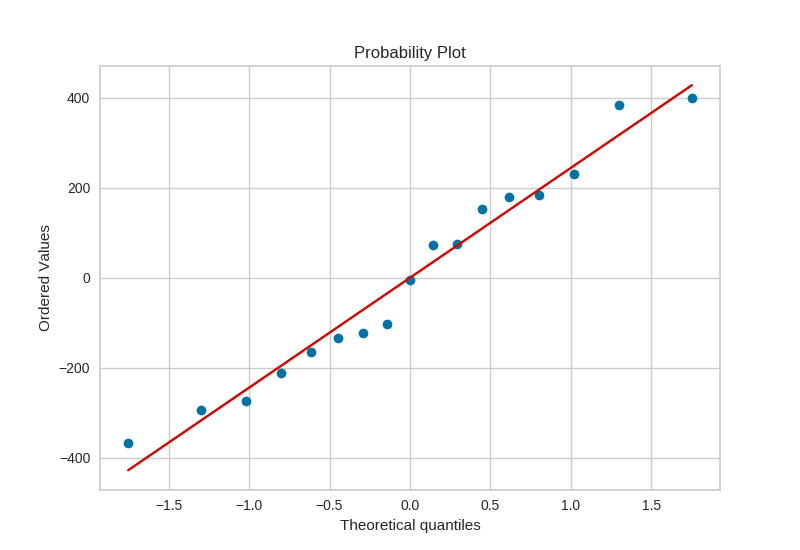
\includegraphics[width=\textwidth]{qq.png}
\caption{QQ-plot of residuals}
\label{figure:1}
\end{figure}

\begin{figure}
\centering
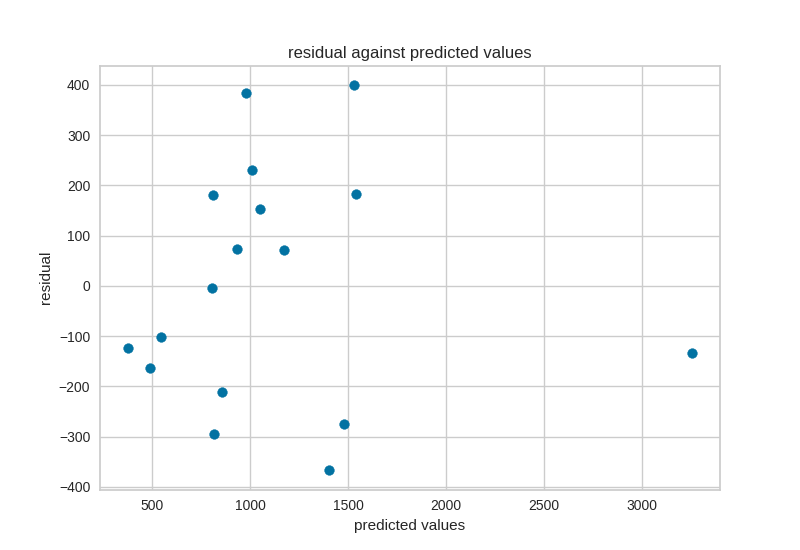
\includegraphics[width=\textwidth]{predicted.png}
\caption{Residuals vs predicted values}
\label{figure:2}
\end{figure}

\begin{figure}
\centering
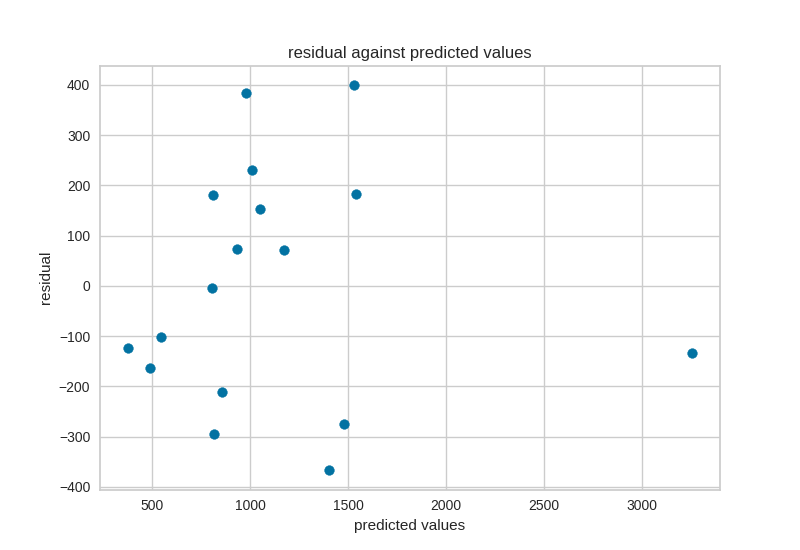
\includegraphics[width=\textwidth]{predicted.png}
\caption{Residuals vs products of predictor values}
\label{figure:3}
\end{figure}

\begin{figure}
\centering
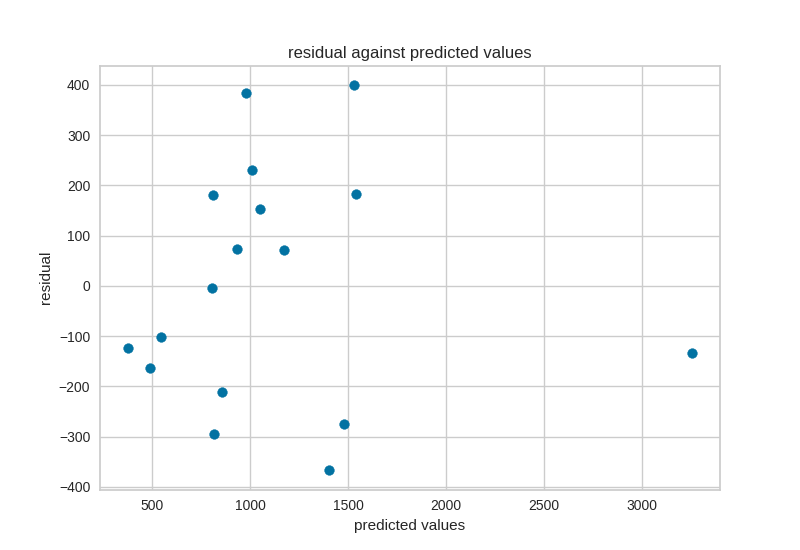
\includegraphics[width=\textwidth]{predicted.png}
\caption{Residuals vs sample numbers}
\label{figure:4}
\end{figure}

\item (iii) The confidence intervals for the new data is $[41.35, 1417,70]$
\end{itemize}
\end{document}






